\documentclass[10pt,a4paper]{article}
\usepackage{graphicx}
\usepackage{subfig}
\usepackage{wrapfig}


\begin{document}


\section{Related work}
\begin{figure}[ht!]
    \centering
    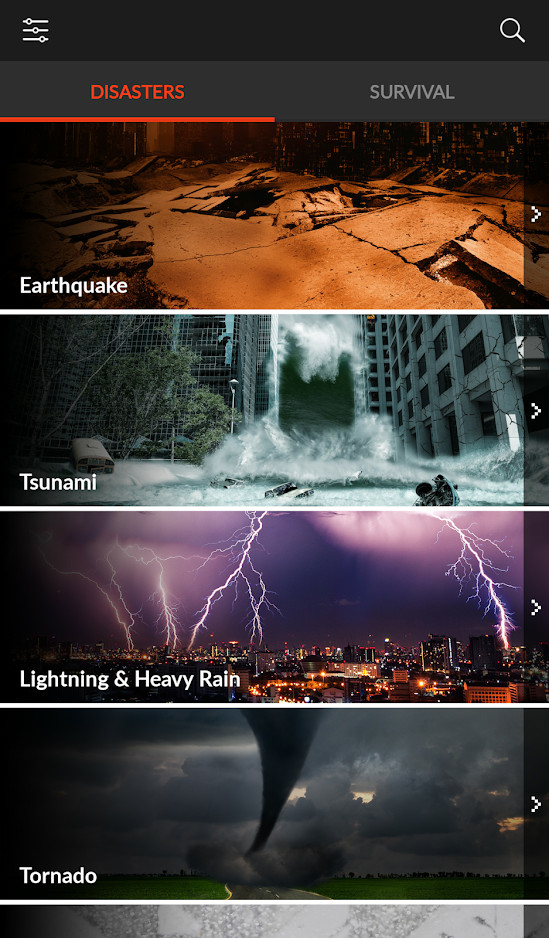
\includegraphics[height=7cm]{appImages/EPD1.jpg}
    \qquad
    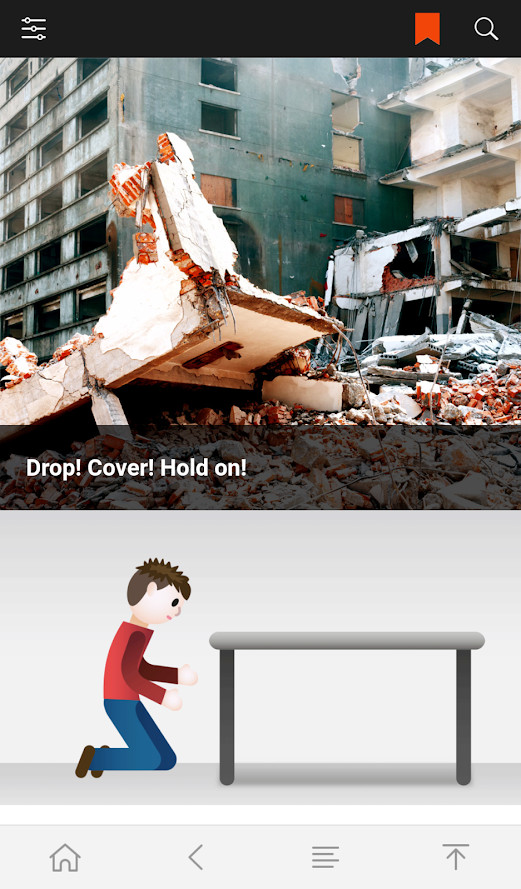
\includegraphics[height=7cm]{appImages/EPD2.jpg}
    \caption{Emergency preparedness \& Disaster Survival Guide is paid mobile application that cover almost all the how to survive a disastrous situation with simple  illustrations and written guides.}%
    \label{fig:example}%
\end{figure}

   
\begin{figure}[ht!]
    \centering
    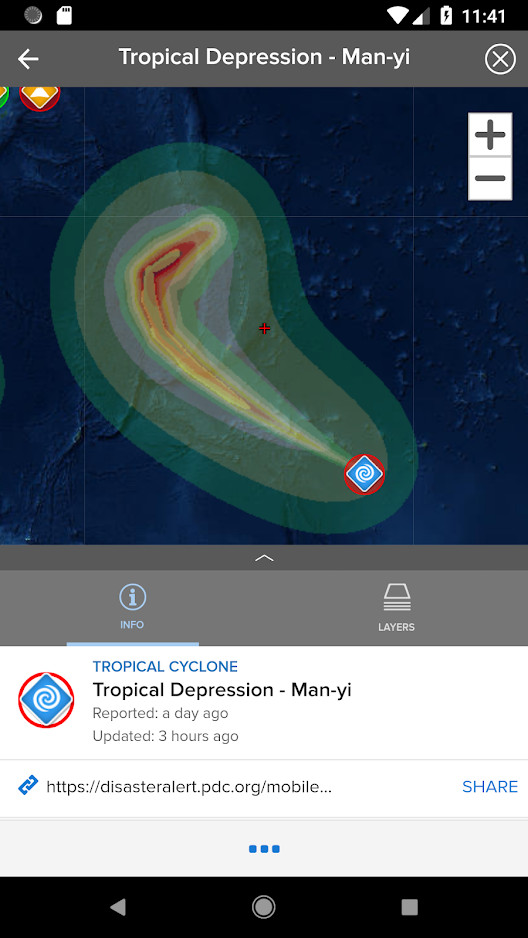
\includegraphics[height=7cm]{appImages/DA1.jpg}
    \caption{Disaster Alert is a free, mobile app that provides individuals, families, and their loved ones with the information they need to stay safe anywhere in the world. Disaster Alert offers near real-time updates about 18 different types of active hazards as they are unfolding around the globe.}
    \label{fig:my_label}
\end{figure}

\section{Design and Implementation Constraints}

\subsection{Solution Constraints}
Due to the choice of technology, some constraints have arisen mainly in the web crawling section. To start, a crawler must wait between repeated accesses to the same website. Otherwise, the crawler can be blocked. In addition, duplicate content can generate a waste of valuable resources.

\subsection{Memory \& Space Constraints}
Our application run on mobile devices with very limited hardware specs which may lead to overheating or battery drain, above all that it will be limited to small amount of ram and storage space on some devices. 

\subsection{Schedule Constraints}
The project has a relatively small time-frame. Therefore, the time is a major concern. The project should be functioning and completed by the mid of 2019.

\subsection{Policy constrains}
The application tries to use all the available mobile resource in disastrous times to save all the user in potential danger eg: using the phone while it's on standby mode to alert the user or use mobile flash to help users who are stuck under derbies. Although we do our best to save the user life, this does not mean we will prevent their death 100\%, which is must be stated to clear us from any charges.
\end{document}

 